\subsection{Progettazione della Technology Baseline}
A causa della concomitanza con la sessione accademica, il team ha fissato la prima \glo{milestone} al termine di questo periodo. 
\subsubsection{Obiettivi}
Il gruppo dovrà aver iniziato lo studio delle tecnologie per la \textit{Technology Baseline}, oltre ad aver controllato buona parte della documentazione.
\subsubsection{Periodi e attività}
Questo periodo è unico e ha inizio il giorno 18-01-2021, successivamente alla revisione dei requisiti, con termine fissato per il giorno 07-02-2021. Comprende attività di: 
\begin{itemize}
\item \textbf{Incremento e verifica dei documenti}: se fosse necessario, i documenti prodotti dal team verranno integrati;
\item \glo{\textbf{Technology Baseline}}: viene fatta un'analisi ad alto livello per comprendere le tecnologie coinvolte.
\end{itemize}

\begin{figure}[h]
	\centering	
	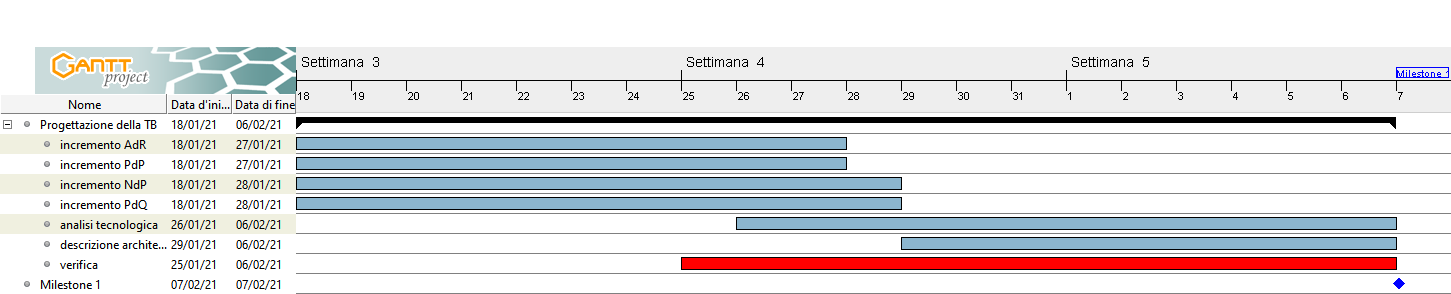
\includegraphics[width=\linewidth]{Images/GanttPianificazioneProgettazioneTB.PNG}
	\caption{Diagramma di Gantt dell'attività di progettazione della Technology Baseline}
\end{figure}